\documentclass[a4paper,11pt]{article}

\usepackage{graphicx}
\usepackage[utf8]{inputenc}
\usepackage[francais]{babel}
\usepackage{amsmath}
\usepackage[T1]{fontenc}
\usepackage{setspace}

\setstretch{1.3}
\setlength{\parindent}{0in}
\baselineskip=30pt

\title{Microcorruption.com Write-up}
\author{David Wong}
\date{7 Décembre 2014}

\begin{document}

\maketitle

\section{Level 1: Tutorial}\label{level-1-tutorial}

Just follow the tutorial :)

\section{Level 2: New Orleans}\label{level-2-new-orleans}

\begin{figure}[htbp]
\centering
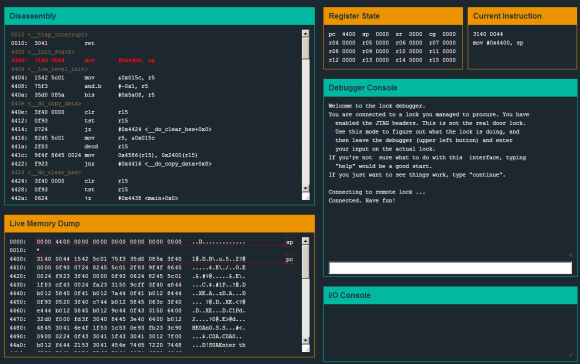
\includegraphics{img/1_1.png}
\caption{micro corruption}
\end{figure}

\href{http://microcorruption.com/}{MicroCorruption} is a ``game'' made
by \textbf{Matasano} in which you will have to debug some programs in
\textbf{assembly}. There is a total of 19 levels and each one is harder
and harder. The first levels are made for begginners though! So it seems
like a great tool to learn.

I didn't know anything about \textbf{asm} (assembly) prior to this so I
will try to document my journey in this challenge.

\textbf{Level 1, New Orleans} is supposed to be easy.

MicroCorruption comes with a nice debugger. Writing \texttt{c} (as
\emph{continue}) in the \textbf{debugger console} runs the program and
allows you to try a password.

\begin{figure}[htbp]
\centering
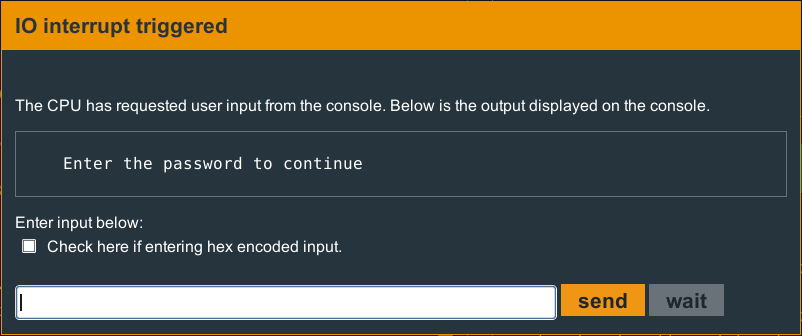
\includegraphics{img/1_2.png}
\caption{password}
\end{figure}

Of course entering \emph{password} doesn't work. let's type
\texttt{reset} in the console and try again. The debugger creates a
\textbf{breaking point} automatically after the pop-up.

After a few \texttt{n} (next instruction) we end up in a
\texttt{check\_password} function. Obviously it is checking if the
password is correct. This is where it starts.

\begin{figure}[htbp]
\centering
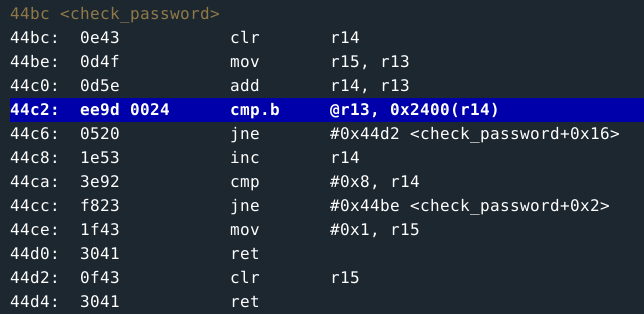
\includegraphics{img/1_3.png}
\caption{e}
\end{figure}

Some explanations on the window:

\begin{itemize}
\item
  on the left you can see the addresses in the memory of each
  instructions. They are written in base 16 (1 means 8bits) and each
  instruction seems to take a different size.
\item
  after this you can see the instruction written in hexadecimal
  directly. It's not very useful, at least at this level.
\item
  then you have the instruction that consists of an \textbf{opcode}
  (\texttt{clr} on the first line) along with its \textbf{arguments}.
\end{itemize}

What the function does is basically this:

\begin{Shaded}
\begin{Highlighting}[]
\NormalTok{r14 = }\DecValTok{0}\NormalTok{;}
\NormalTok{r13 = r15; }\CommentTok{// r13 points to something}
\NormalTok{r13 += r14; }\CommentTok{// we add r14 to the address in r13}
\KeywordTok{if}\NormalTok{(*r13 == *(}\BaseNTok{0x2400} \NormalTok{+ r14))\{}
    \NormalTok{r14++;}
    \KeywordTok{if}\NormalTok{(r14 != }\DecValTok{8}\NormalTok{)\{}
        \CommentTok{// go back to the r13 += r14 line}
    \NormalTok{\}}
    \KeywordTok{else}\NormalTok{\{}
        \NormalTok{r15 = }\DecValTok{1}\NormalTok{;}
        \KeywordTok{return}\NormalTok{;}
    \NormalTok{\}}
\NormalTok{\}}
\KeywordTok{else}\NormalTok{\{}
    \NormalTok{r15 = }\DecValTok{0}\NormalTok{;}
    \KeywordTok{return}\NormalTok{;}
\NormalTok{\}}
\end{Highlighting}
\end{Shaded}

\begin{quote}
So we compare what's in r13 with what's in address 0x2400.\\Then we
compare the next byte, and on and on for 7 bytes.
\end{quote}

We can see later in the code that if \texttt{r15 = 0} it's a bad thing,
and if it equals \texttt{1} then we're done!\\At this point we can
easily guess that what is at the address 0x2400 and of length 7 bytes
must be the password.

\begin{figure}[htbp]
\centering
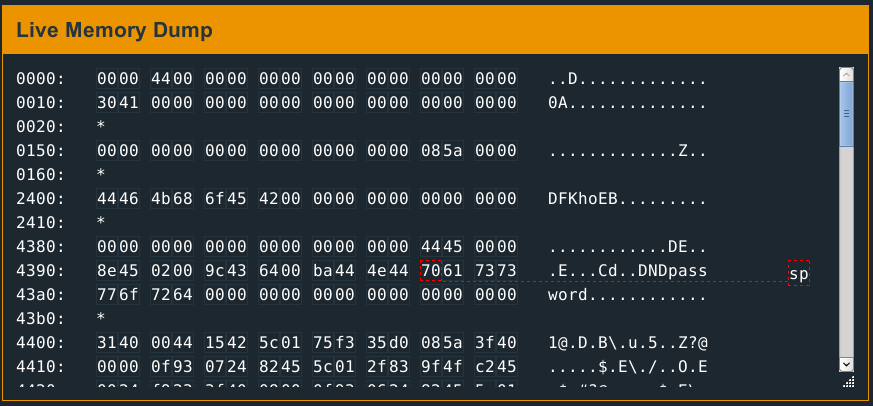
\includegraphics{img/1_4.png}
\caption{f}
\end{figure}

The live \textbf{memory dump} gives us a string. We enter it as the
password: it works!\\We couldn't see that without running the program
because the password was created during runtime, we can see the function
that does that here:

\begin{figure}[htbp]
\centering
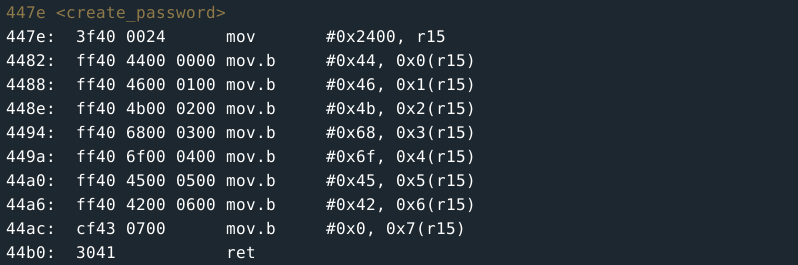
\includegraphics{img/1_5.png}
\caption{g}
\end{figure}

\section{Level 3: Sydney}\label{level-3-sydney}

Level 2 here we come!

Let's quickly check the code, we can spot that it's the same as level 1.
We have a \texttt{check\_password} function that has to change
\texttt{r15} to something which is not zero.

\begin{figure}[htbp]
\centering
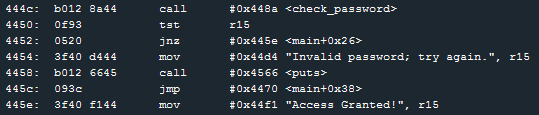
\includegraphics{img/2_1.PNG}
\caption{microcorruption}
\end{figure}

Alright let's look at \texttt{check\_password} shall we?

\begin{figure}[htbp]
\centering
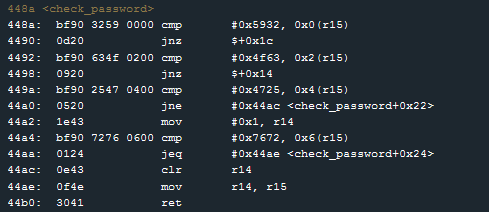
\includegraphics{img/2_2.PNG}
\caption{microcorruption}
\end{figure}

So \texttt{0x5932} (the \texttt{0x} part means we write in hexadecimal!)
is getting compared against r15. Since \textbf{MSP430} is 16bits,
instructions like cmp compare 16bits by default.\\Then we compare
\texttt{0x4f63} with \texttt{0x2(r15)} which means the content at
address r15 + 2 bytes.\\And on and on. Bad comparisons at every step
makes the program jumps and set r15 to zero which we don't want.

Note that there are two different jumps here: * Relative jumps:
\texttt{jnz \$+0x14} (using the relative instruction located at
``current instruction + 0x14'') * Absolute jumps: \texttt{jne \#0x44ac}
(using the absolute address of the instruction ``0x44ac'')

Note number 2: * jnz: Jump if not zero. If the previous comparison
checks it should change some flag to zero and the jnz should not work. *
jne: Jump if not equal. Same principle.

At this point we could \textbf{guess} that the password is something
like \emph{0x59324f6347257672}

Well. Curiously this does not work. After a bit of research, maybe we
are in \href{http://en.wikipedia.org/wiki/Endianness}{little-endian}?

Trying \emph{0x3259634f25477276} it works!

Basically what the \texttt{cmp} opcode does is slicing the 2 bytes we
feed it in chunks of size 1 byte and ordering them accordingly to our
system's endianness. So here it would be in reverse order.

\section{Level 4: Hanoi}\label{level-4-hanoi}

We know how this works now, let's go straight for the \emph{``That
password is not correct.''} line. Scrolling through the {[}code{]} we
can see that a comparison of byte between the value \texttt{0xe0} (224)
and the content at address \texttt{0x2410}, if it is not equal the
program jumps to address login+0x50. In the Debugger Console we type
\texttt{r login+50} to read the memory at this address. We can see that
it is indeed the line 4570 of the memory which is our \emph{``That
password is not correct.''} line.

\begin{figure}[htbp]
\centering
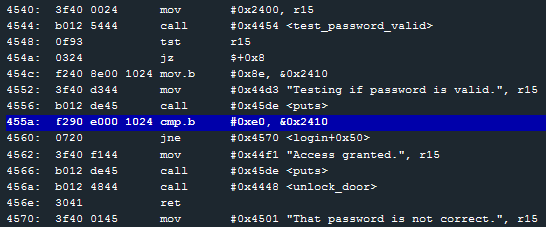
\includegraphics{img/3_1.PNG}
\caption{image}
\end{figure}

We see that just a few steps ahead, the code sets the byte at
\texttt{0x2410} to \texttt{0x8e}. That is different from \texttt{0xe0}
so the test will inconditionnally fail. Fortunatelly this is avoided if
we jump this instruction. That's exactly what is happening if
\texttt{tst r15} works. Does it?

\begin{itemize}
\itemsep1pt\parskip0pt\parsep0pt
\item
  I set a break point in this instruction with \texttt{b 454a}.
\item
  I run the program with \texttt{c} until it goes to my breakpoint.
\item
  I then \texttt{step} instructions to see that it does makes the jump
  eventhough I entered an incorrect password.
\end{itemize}

So the \texttt{mov.b \#0x8e, \&0x2410} line is just here to confuse.

\subsection{test\_password\_valid}\label{testux5fpasswordux5fvalid}

Just before calling \texttt{test\_password\_valid} (that seems to be the
function that checks for the correctness of our password) we seem to
move the value \texttt{0x2400} in the \texttt{r15} register. What's
there?

\begin{itemize}
\itemsep1pt\parskip0pt\parsep0pt
\item
  I set a break point in this instruction with \texttt{b 4540}
\item
  I run the program with \texttt{c}
\item
  I enter some dumb value in the password field and I continue to my
  breakpoint
\item
  Once I'm there I check what's in 0x2400 with \texttt{r 2400}, I get
  the dumb value I entered.
\end{itemize}

So \texttt{r15} contains the address where the password I entered is
located. \texttt{2400} is the address where the password is located.

\subsection{what if?}\label{what-if}

What if I entered a password long enough to reach the address
\texttt{2410} so I could put the \texttt{0xe0} value there and my work
would be done?

\begin{quote}
Let's remember. An address contains 1 byte, so we have to write 1 byte
of password to reach the next address. In hexadecimal that's two
letters.
\end{quote}

Let's try to enter \texttt{aaaaaaaaaaaaaaaaaaaaaaaaaaaaaaaae0}.
\textbf{It works!}

\section{Level 5: Cusco}\label{level-5-cusco}

When we entered the level, we are greeted with this a message

\begin{quote}
\begin{itemize}
\itemsep1pt\parskip0pt\parsep0pt
\item
  We have fixed issues with passwords which may be too long.
\end{itemize}
\end{quote}

That's a reference to level 3 :)

\subsection{Let's start}\label{lets-start}

We see that if we try to enter a long password it stores a maximum of
48bytes of it in the stack.

\begin{quote}
aaaaaaaaaaaaaaaaaaaaaaaaaaaaaaaaaaaaaaaaaaaaaaaaaaaaaaaaaaaaaaaaaaaaaaaaaaaaaaaaaaaaaaaaaaaaaaaa
\end{quote}

We also see that if we continue executing the program with such a long
password it stops running correctly after line \texttt{453e} which is
the return instruction \texttt{ret} of the function \texttt{login}. It
seems we have overwrote the instructions. A quick of the program counter
(\texttt{r pc 8}) to read the next instruction shows that there are all
zeros.

The \texttt{ret} instruction of a function takes the last value in stack
and loads it into the Program Counter \texttt{pc}
(\href{http://en.wikipedia.org/wiki/Program_counter}{also called the
Instruction Pointer \texttt{ip} in intel x86}). What we did was
overwriting the stack (\textbf{stack overflow}) and changing the
\textbf{return value} of the function, which was supposed to be the next
instruction.

\subsection{Where is the value we have to
change?}\label{where-is-the-value-we-have-to-change}

Okay, so where exactly is this value we had to change? I will enter
``password'' as password so I can quickly find it in the memory, and
break on the \texttt{ret} instruction so I know where in the stack it
will take its next value (\texttt{b 453e}).

\begin{figure}[htbp]
\centering
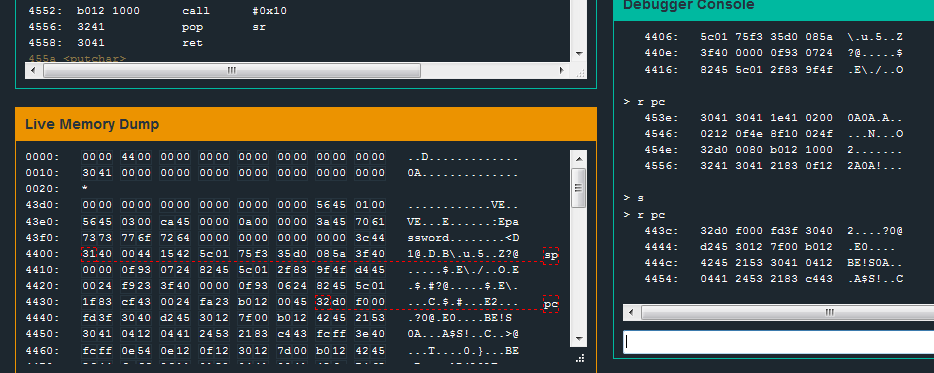
\includegraphics{img/4_1.PNG}
\caption{image}
\end{figure}

Here we see that \texttt{pc} was pointing to \texttt{453e}, and after
the return it points to qddress \texttt{443c} in memory, which was
indeed the last 16bits entry of the stack, located 8bytes after our
``password'' (we can see that in the Live Memory Dump). Now we know that
if we enter a password where the 16th byte is 0xaabb, the program will
load the instruction located at address 0xbbaa in memory (remember, we
are in little endian).

\subsection{What should we load?}\label{what-should-we-load}

What about that function called \texttt{unlock\_door}? Let's try to jump
to that and see if it does what it says.

Let's try with that password:
\texttt{0xaaaaaaaaaaaaaaaaaaaaaaaaaaaaaaaa4644}

\textbf{It works!}

\section{Level 6: Reykjavik}\label{level-6-reykjavik}

\subsection{Quick look}\label{quick-look}

We run the program and hodiho! It seems like at one point our
\texttt{pc} gets lost and doesn't follow the initial path.

Entering a large number of \emph{a} we see that they get stored at
address \texttt{43da} in memory and that we can enter a maximum of 62
a's (15bytes + 2 bits).

\subsection{Encryption}\label{encryption}

If you look at the code, you can see that all \texttt{enc} does is
looping and modifying bits of memory. Basically what it does is
\textbf{building instructions} that we will read afterward by
\textbf{pointing the Program Counter on them}. It's mostly
incomprehensible so let's not waste time with this. \texttt{r pc 100}
gives us the hexadecimal code that we can then Disassemble through
Microcorruption Disassembler, or we can just step through it and observe
what is really happening through the Current Instruction window.

\begin{figure}[htbp]
\centering
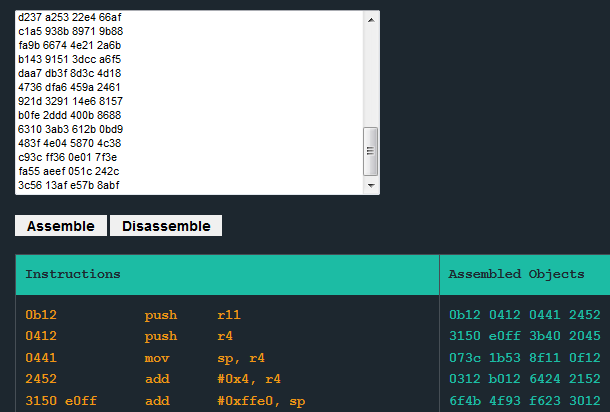
\includegraphics{img/5_1.PNG}
\caption{disassembler}
\end{figure}

We step through the code until we get prompted by the pop-up asking for
a password. We can then check that it gets saved into the stack
(\texttt{r sp}).

Right after the popup, this code appears:

\texttt{b490 b26b dcff cmp \#0x6bb2, -0x24(r4)}

The instruction compares \texttt{0x6bb2} with what is at the address
pointed by r4, minus 24 bytes. Magically, this where our password is
stored. Remember, \textbf{the instruction \texttt{cmp} compares 16bits
in MSP430}, so the password starts like this: \texttt{0xb26b} (remember
we are in \textbf{little endian}!). Stepping through the code we don't
see anymore \texttt{cmp}. Let's try this value as a password. \textbf{It
works!}

\section{Level 7: Whitehorse}\label{level-7-whitehorse}

\subsection{Quick look}\label{quick-look-1}

We quickly test our program and see that we can enter a password of
maximum 48bytes and that we have a \textbf{stack overflow} after a
length of 16 bytes.

The Program jumps to the address located in the bytes number 17 and 18
of our password, this occurs after the Interrupt that checks our
password.

\subsection{Where should we jump?}\label{where-should-we-jump}

The program uses HSM-2 to check the password. We don't have access to
it. In the LockIT Pro \textbf{Manual} we can read:

\begin{quote}
\textbf{INT 0x7F.} Interface with deadbolt to trigger an unlock if the
password is correct. Takes no arguments
\end{quote}

We just have to call an 0x7F interrupt. To tell that to the program we
have to simulate the \texttt{push \#0x7F} so that the interrupt would
work.

If we enter this password: \emph{aaaaaaaaaaaaaaaaaaaaaaaaaaaaaaaa60447f}

When the \texttt{ret} will occurs, it will put 4460 inside \texttt{pc}
and points the Stack Pointer \texttt{sp} to the value 7f. That's exactly
what we want, and it works.

\section{Level 8: Montevideo}\label{level-8-montevideo}

\subsection{Quick Look}\label{quick-look-2}

We can enter a 3x16bytes password (same as previous level). The program
uses strcpy and memset (this is new). We have a stack overflow after 16
bytes (like the previous level). So let's try entering the exact same
password \emph{aaaaaaaaaaaaaaaaaaaaaaaaaaaaaaaa60447f}.

It works\ldots{}

(I think it comes from the use of strcpy, it copies until it finds a \0
but we can still overflow the stack, buffer overflow, particularly a
stack overflow. This is stack smashing because we change the RIP (return
instruction pointer) here maybe it would be called RPC (return program
counter?))

(The function copies a supplied string without bounds checking by using
strcpy() instead of strncpy().
(http://insecure.org/stf/smashstack.html))

\section{Level 9: Johannesburg}\label{level-9-johannesburg}

\subsection{Quick Look}\label{quick-look-3}

There is now a security against passwords that exceed a certain number
of letters, but the security happens after storing it in stack so we can
still store a longer password than expected. The maximum possible seems
to be 37bytes. But the last \texttt{ret} is avoided by a \texttt{br}
(branch to destination) and the program is shut down early, so no stack
overflow here.

\subsection{How is the password's length
checked?}\label{how-is-the-passwords-length-checked}

\begin{figure}[htbp]
\centering
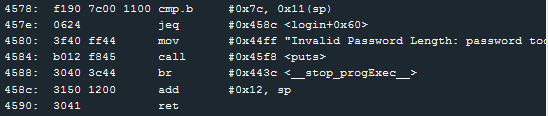
\includegraphics{img/8.PNG}
\caption{password check}
\end{figure}

Seems like a password of length superior than 17 bytes is too much, to
test the security of this it just checks if the value located after the
17byte password in the stack is 0x7c, a value that is supposed to be
here. \texttt{cmp.b   \#0x7c, 0x11(sp)}

Here's the trick, if we set the 18th byte of our password to 0x7c then
it will work!

We can then jump to the call interrupt and set the last byte of the
stack to 0x7f like we did in the previous levels:

the password \emph{aaaaaaaaaaaaaaaaaaaaaaaaaaaaaaaaaa7c6c447f} works.

\section{Level 10: Santa Cruz}\label{level-10-santa-cruz}

\subsection{First protection}\label{first-protection}

We try entering a long username and password and we get directly kicked
out of the program at line 460c. The program seems to check address
r4-19 (0x43b3) and compare it with r11. If it doesn't match then it
exits.

\textbf{The r11 register seems to hold the password length.}

\begin{figure}[htbp]
\centering
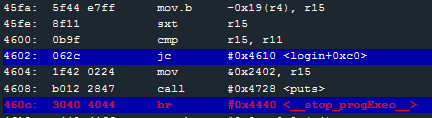
\includegraphics{img/10_1.PNG}
\caption{image}
\end{figure}

\texttt{jc} Jump on Carry, similar to Jump if Below (\emph{JB}) or Jump
if Not Above or Equal (\texttt{JNAE})

We can circumvent that if what is at address \texttt{0x43b3} is
\textbf{below than the password's length}.

We check this address to see that it's overflowed by the
\textbf{username} we entered. We can set the 18th byte of the username
to something lower than the password length and it will pass the test.

\begin{figure}[htbp]
\centering
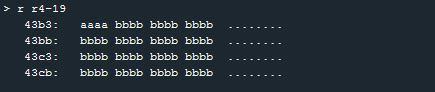
\includegraphics{img/10_2.PNG}
\caption{image}
\end{figure}

\begin{quote}
here I entered a series of \emph{a}'s as username, and a series of
\emph{b}'s as password.
\end{quote}

\subsection{Second protection}\label{second-protection}

We get kicked a second time but at a different line (45f6).

\begin{figure}[htbp]
\centering
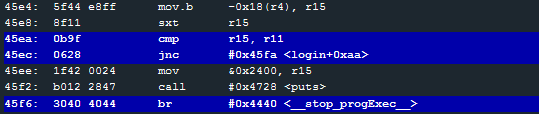
\includegraphics{img/10_3.PNG}
\caption{second protection}
\end{figure}

\texttt{jnc} Jump No Carry, equivalent to Jump if Not Below (JNB) or
\textbf{Jump if Above or Equal} (JAE). So we jump if the byte at address
\texttt{0x43b4} \textbf{is not below the password's length}. This
address can be modified by the 19th byte of the username.

\begin{quote}
Note that the initial values are respectively 8 and 10, meaning that
they expected us to enter a password greater than 8 and lesser than 11
characters.
\end{quote}

\subsection{Third protection}\label{third-protection}

We get halted one last time at line 0x465a.

\begin{figure}[htbp]
\centering
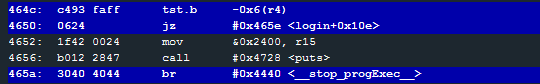
\includegraphics{img/10_4.PNG}
\caption{third protection}
\end{figure}

\texttt{tst.b -0x6(r4)}: if the byte at address r4 - 6 (\texttt{0x43c6})
is not zero, it will exit. (canary) It is the 18th byte of the password
we entered.

Thus, this combination of username and password should pass the three
tests we described:

username: aaaaaaaaaaaaaaaaaaaaaaaaaaaaaaaaaa01ff password:
bbbbbbbbbbbbbbbbbbbbbbbbbbbbbbbbbb00bbbbbb {[}\ldots{}{]} bbbb

\subsection{Stack Overflow}\label{stack-overflow}

We passed all the test and couldn't produce a stack overflow with the
password. Did I miss something? Let's try with the username

username: aaaaaaaaaaaaaaaaaaaaaaaaaaaaaaaaaa01ffaaa {[}\ldots{}{]} aaa
password: bbbbbbbbbbbbbbbbbbbbbbbbbbbbbbbbbb00

That's the solution. The Stack Pointer points to some remains of the
username right before executing the last \texttt{ret} of our program. We
can now do a stack overflow by modyfing the 43th byte of the username to
the address we want to jump to.

We use the 7F call interrupt technique of the previous challenge.

username:
aaaaaaaaaaaaaaaaaaaaaaaaaaaaaaaaaa01ffaaaaaaaaaaaaaaaaaaaaaaaaaaaaaaaaaaaaaaaaaaaaaa72447f
password: bbbbbbbbbbbbbbbbbbbbbbbbbbbbbbbbbb00

\textbf{It works!}

\section{Level 11: Jakarta}\label{level-11-jakarta}

\subsection{First protection}\label{first-protection-1}

Entering different usernames we see that \textbf{r11 is the username's
length}. Look at the instruction \texttt{cmp.b \#0x21, r11}

\begin{figure}[htbp]
\centering
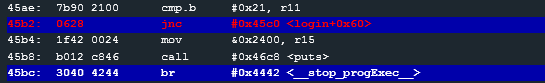
\includegraphics{img/11_1.PNG}
\caption{first protection}
\end{figure}

\begin{quote}
\texttt{jnc} \textasciitilde{} Jump if Above or Equal
\end{quote}

So we pass the first test if \textbf{the username's length is lesser
than 33 bytes} (0x21).

\subsection{Second protection}\label{second-protection-1}

\begin{figure}[htbp]
\centering
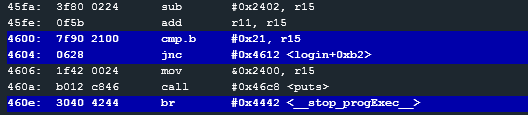
\includegraphics{img/11_2.PNG}
\caption{second protection}
\end{figure}

\texttt{add r11, r15} \texttt{cmp.b \#0x21, r15} \texttt{jnc}

So \textbf{the sum of the username and the password lenghts} have to be
lesser than 33 bytes as well (0x21).

\subsection{Stack Overflow}\label{stack-overflow-1}

\begin{figure}[htbp]
\centering
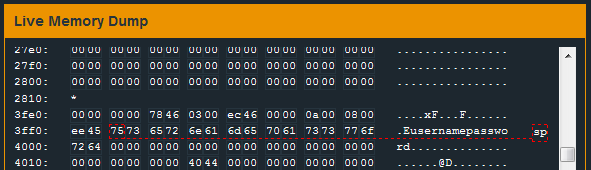
\includegraphics{img/11_3.PNG}
\caption{stack}
\end{figure}

We see that the username and the password are stored in the stack thanks
to the \texttt{strcpy}.

\begin{figure}[htbp]
\centering
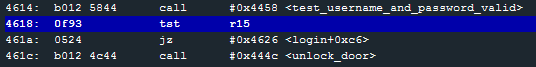
\includegraphics{img/11_4.PNG}
\caption{test}
\end{figure}

We see that the password is tested in the function
\texttt{test\_username\_and\_password\_valid} through the 7d interrupt.
So we cannot do anything here. It is obvious we need to create a stack
overflow again.

But let's go back to our previous tests

\begin{figure}[htbp]
\centering
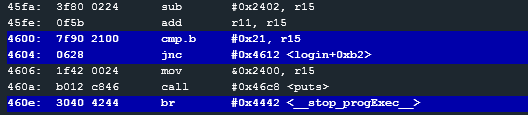
\includegraphics{img/11_2.PNG}
\caption{second protection}
\end{figure}

Don't you see something? \texttt{cmp.b \#0x21, r15}. This means: compare
byte of r15 and 0x21. But words are 2 bytes in MSP430 (so registers and
address in the stack are 2 bytes). What if we wrote 0x1020 for example.
Would it be lesser than 0x21 ?

Let's try that.

I enter
\texttt{aaaaaaaaaaaaaaaaaaaaaaaaaaaaaaaaaaaaaaaaaaaaaaaaaaaaaaaaaaaaaaaa}
(length of 0x20) as username.

we want the toal to be 0x0100 to test our hypothesis. So we need 0xd0
more (14 * 16 = 224 bytes).

Entering
\texttt{bbbbbbbbbbbbbbbbbbbbbbbbbbbbbbbbbbbbbbbbbbbbbbbbbbbbbbbbbbbbbbbbbbbbbbbbbbbbbbbbbbbbbbbbbbbbbbbbbbbbbbbbbbbbbbbbbbbbbbbbbbbbbbbbbbbbbbbbbbbbbbbbbbbbbbbbbbbbbbbbbbbbbbbbbbbbbbbbbbbbbbbbbbbbbbbbbbbbbbbbbbbbbbbbbbbbbbbbbbbbbbbbbbbbbbbbbbbbbbbbbbbbbbbbbbbbbbbbbbbbbbbbbbbbbbbbbbbbbbbbbbbbbbbbbbbbbbbbbbbbbbbbbbbbbbbbbbbbbbbbbbbbbbbbbbbbbbbbbbbbbbbbbbbbbbbbbbbbbbbbbbbbbbbbbbbbbbbbbbbbbbbbbbbbbbbbbbbbbbbbbbbbbbbbbbbbbbbbbbbbbbbbbbbbbbbbbbbbbbbbbbbbbbbb}
it works and we get lost at a random address. We've successfully
overwrote the return address.

Breaking on the return instruction we can see at what address the Saved
PC is (at the SP address).

\begin{figure}[htbp]
\centering
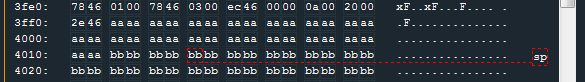
\includegraphics{img/11_5.PNG}
\caption{seip}
\end{figure}

So we can enter our personalized return address at the byte number 5 and
6 of our password (if our username is of length 0x20 of course). Let's
return at the instruction \texttt{unlock\_door}.

So entering the same username, and this as password works:

\texttt{bbbbbbbb1c46bbbbbbbbbbbbbbbbbbbbbbbbbbbbbbbbbbbbbbbbbbbbbbbbbbbbbbbbbbbbbbbbbbbbbbbbbbbbbbbbbbbbbbbbbbbbbbbbbbbbbbbbbbbbbbbbbbbbbbbbbbbbbbbbbbbbbbbbbbbbbbbbbbbbbbbbbbbbbbbbbbbbbbbbbbbbbbbbbbbbbbbbbbbbbbbbbbbbbbbbbbbbbbbbbbbbbbbbbbbbbbbbbbbbbbbbbbbbbbbbbbbbbbbbbbbbbbbbbbbbbbbbbbbbbbbbbbbbbbbbbbbbbbbbbbbbbbbbbbbbbbbbbbbbbbbbbbbbbbbbbbbbbbbbbbbbbbbbbbbbbbbbbbbbbbbbbbbbbbbbbbbbbbbbbbbbbbbbbbbbbbbbbbbbbbbbbbbbbbbbbbbbbbbbbbbbbbbbbbbbbbbbbbbbbbbbbbbb}

\section{Level 12: Addis Ababa}\label{level-12-addis-ababa}

\begin{figure}[htbp]
\centering
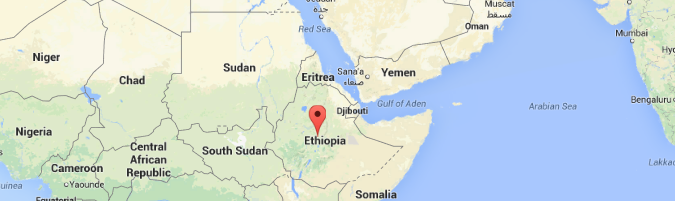
\includegraphics{img/12_1.PNG}
\caption{addis ababa}
\end{figure}

\subsection{Quick observations}\label{quick-observations}

\begin{itemize}
\itemsep1pt\parskip0pt\parsep0pt
\item
  The password is tested through \texttt{test\_password\_valid} with a
  7d interrupt (HSM Model 1).
\item
  We have an \texttt{unlock\_door} function (so no need to go through
  the \texttt{test\_password\_valid} function if we can return to
  it).(44da)
\item
  We have no \texttt{ret} after the main (so we can't modify the return
  address).
\item
  If the SP is different from zero the program unlocks the doors.
\item
  We have a printf of our username (\textbf{format string
  vulnerability}!)
\end{itemize}

\subsection{Printf in Manual}\label{printf-in-manual}

\begin{figure}[htbp]
\centering
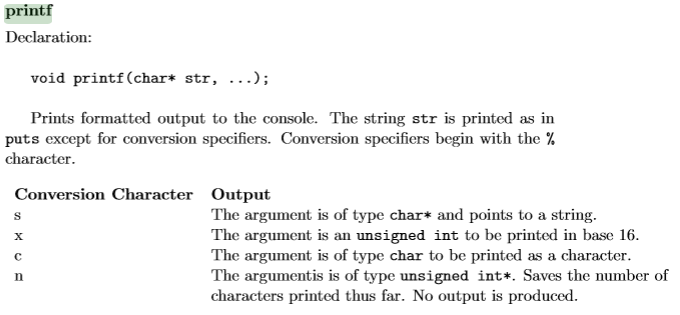
\includegraphics{img/12_2.PNG}
\caption{printf}
\end{figure}

We see that printf is a limited version of the C equivalent. Since we
have \%n available we know we can write to the memory and thus we should
be able to do a Format String exploit.

\begin{figure}[htbp]
\centering
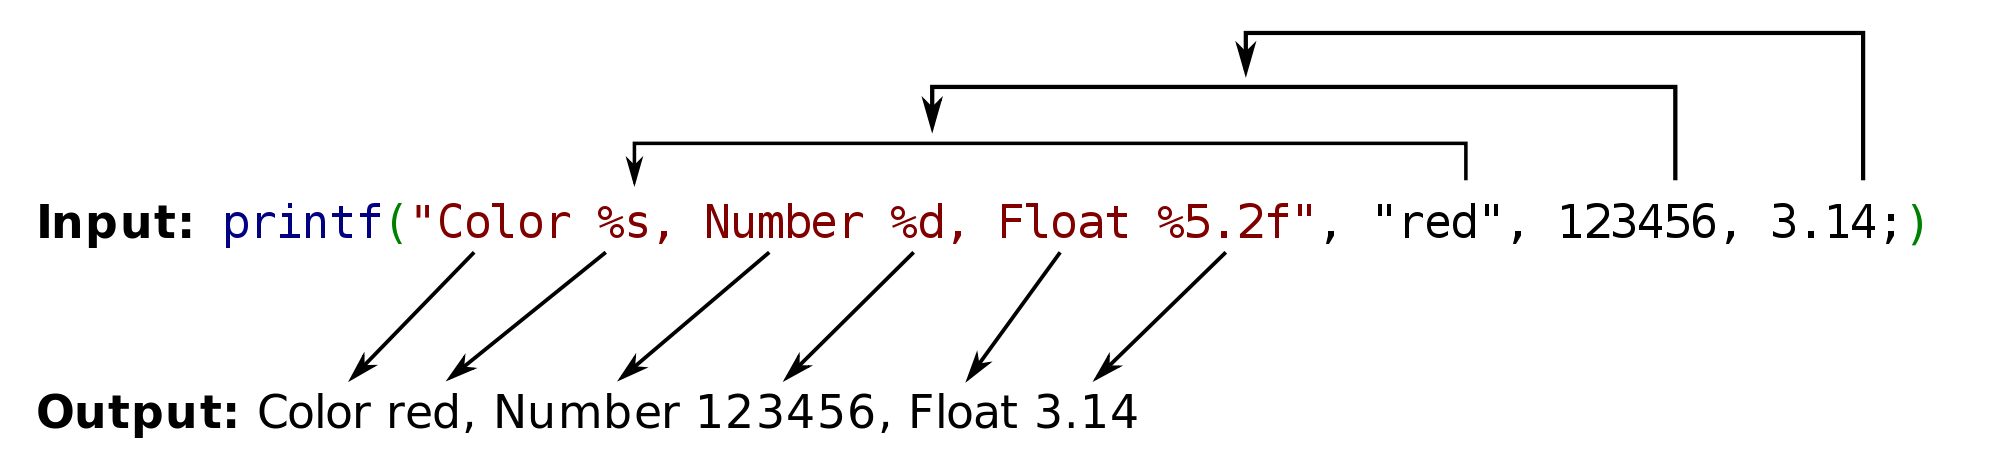
\includegraphics{img/12_3.PNG}
\caption{printf}
\end{figure}

So here the developer did a:

\texttt{printf(user\_input);}

instead of this:

\texttt{printf("\%s", user\_input);}

So the user\_input becomes the format string and it will look in the
stack for its arguments (in the example red, 123456, and \ldots{} are
pushed in the stack).

\subsection{Printf in MSP430}\label{printf-in-msp430}

Let's try \texttt{\%x} as input. It doesn't output anything. So the
first argument must be null:

\texttt{printf(user\_input, 0x00);}

Let's try again with \texttt{\%x \%x}. It outputs \texttt{7825} which is
\texttt{\%x} reversed (little endian). It seems like when we point to
our second arguments we are pointing to the beginning of our input.
Since a word is 16bits in MSP430 we only display 2 characters in
hexadecimal.

So if we enter \texttt{PTR\%x\%n} we will write 5 to the address in PTR.
note that we can use \%x, \%c, \%n\ldots{} as our first format since we
won't use it.

\subsection{Exploit}\label{exploit}

Remember what we observed at the begginning:

\begin{quote}
If the SP is different from zero the program unlocks the doors.
\end{quote}

\begin{figure}[htbp]
\centering
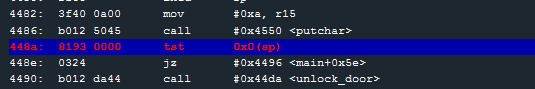
\includegraphics{img/12_5.PNG}
\caption{final}
\end{figure}

It was at this line. And by breaking on it we can see that sp is
pointing to 3062.

So let's try to do \texttt{6230256e256e}

which should write the number of characters printed before the last \%n
(which will be only 2 since the first \%n won't count).

\section{Level 13: Novosibirsk}\label{level-13-novosibirsk}

\begin{figure}[htbp]
\centering
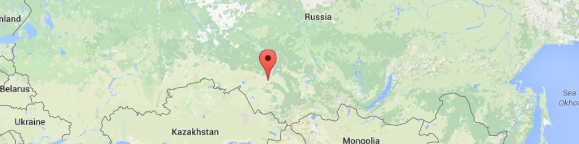
\includegraphics{img/13_1.PNG}
\caption{Novosibirsk}
\end{figure}

\subsection{Observations}\label{observations}

\begin{itemize}
\itemsep1pt\parskip0pt\parsep0pt
\item
  Printf again, except this time the first argument is the user input (a
  simple \texttt{\%x} returns \texttt{7825})
\item
  No main ret.
\item
  Call to \texttt{conditional\_unlock\_door} (HSM-2)
\end{itemize}

\subsection{Format String Again}\label{format-string-again}

The obvious idea here is to change the 7E interrupt to a 7F interrupt.
Let's try the to exploit the Format String to do that.

\begin{figure}[htbp]
\centering
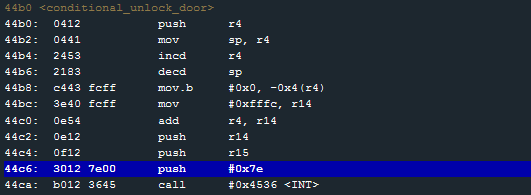
\includegraphics{img/13_2.PNG}
\caption{interrupt}
\end{figure}

So let's build our input: * the address we want to write on (here
\texttt{c844} (little endian)). * Then enough padding to print 7f (127)
bytes including the 4 bytes of the address we're writing on. * The
format \%n

c8446161616161616161616161616161616161616161616161616161616161616161616161616161616161616161616161616161616161616161616161616161616161616161616161616161616161616161616161616161616161616161616161616161616161616161616161616161616161616161616161616161616161256e

This works.

\section{Level 14: Algiers}\label{level-14-algiers}

\begin{figure}[htbp]
\centering
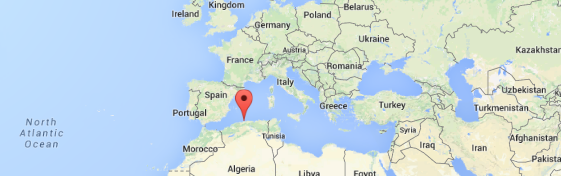
\includegraphics{img/14_1.PNG}
\caption{algiers}
\end{figure}

\subsection{Observations}\label{observations-1}

\begin{itemize}
\itemsep1pt\parskip0pt\parsep0pt
\item
  Use of the \textbf{malloc} function. Hints at a \textbf{Heap Overflow
  Exploit}.
\item
  There are two functions that can unlock this level:
  \texttt{unlock\_door} and \texttt{test\_password\_valid}.
\item
  There seem to be no check on the username and password length. We can
  enter 18 bytes in username and then it gets overwritten by password.
\item
  With a quick test entering a long string of the same letter as
  username and as password we get an error : \textbf{load address
  unaligned: UU75} where UU is the character we entered in the username.
\item
  One character in username input gets changed to ` during the password
  verification (at address 2422 in memory).
\item
  The buffer overflow stops us at line 0x4520 (in the \texttt{free}
  function).
\end{itemize}

\begin{figure}[htbp]
\centering
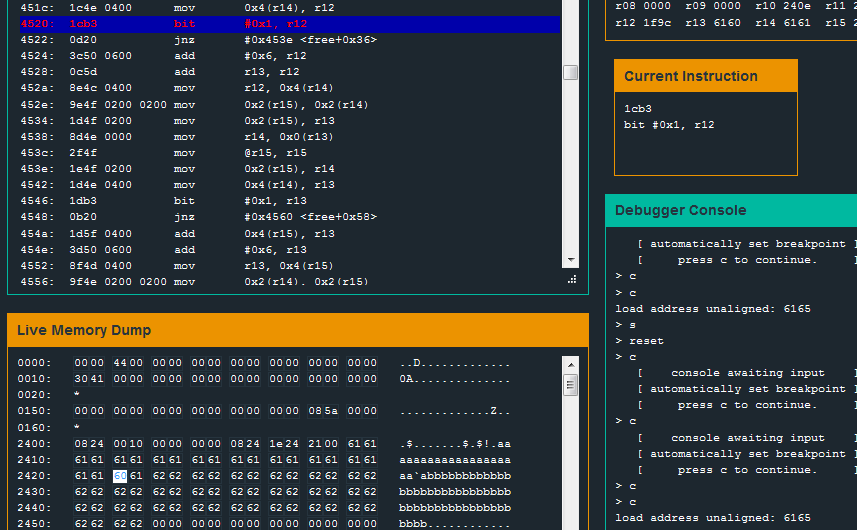
\includegraphics{img/14_2.PNG}
\caption{observations}
\end{figure}

In the Manual we find:

\begin{quote}
BIT arg1 arg2 -\textgreater{} compute arg1 \& arg1, set the flags, and
discard the results (like TEST on x86)
\end{quote}

\subsection{test\_password\_valid}\label{testux5fpasswordux5fvalid-1}

There is a ret at the beggining of the function. Followed by a lot of
strange functions (hints at ROP?)

\end{document}